\lecture{Big data}{14~-~01~-~2026}
%
%
\section{Definizione dei Big Data}
Questa sezione introduce il concetto di Big Data e le problematiche associate alla loro gestione.
Un concetto fondamentale associato ai Big Data è: ``Mai fidarsi dei dati senza averli controllati''.
\begin{itemize}
    \item I dati inseriti manualmente sono poco affidabili e sospetti;
    \item I sensori possono avere guasti sistematici o metadati errati;
    \item È necessario avere una gestione per i dati ``sporchi'' (duplicati, incompleti, in ritardo).
\end{itemize}
%
\subsection{Le 3V dei Big Data}
Il termine nasce dalla difficoltà di immagazzinare ed elaborare dati a causa di tre fattori principali:
\begin{enumerate}
    \item Volume: La quantità di dati sta diventando ingestibile;
    \item Variety (Varietà): La complessità cresce, includendo click stream, sensori, social media, ecc.
    \item Velocity (Velocità): I dati arrivano così rapidamente che devono essere processati istantaneamente o vanno persi.
\end{enumerate}
%
\subsection{Processo di analisi (pipeline)}
Il flusso di lavoro per estrarre valore dai dati segue questi step logici:
\begin{enumerate}
    \item Selezione: Scelta dei dati target;
    \item Preprocessing: Pulizia e preparazione;
    \item Trasformazione: Normalizzazione o modifica per l'analisi;
    \item Data Mining/Analytics: Applicazione di modelli;
    \item Interpretazione/Valutazione: Estrazione di conoscenza (pattern e insight).
\end{enumerate}

%
\section{Architetture dei Big Data e dei Database}
Una problema cruciale che si affronta quando si ha il bisogno di trattare con larghe porzioni di dati è l'adattamento del \emph{software} e dell'\emph{hardware}.

Il problema principale che in cui si incorre è il \emph{bottleneck}, che avviene nel trasferimento dei dati dal disco al processore (per permettere poi l'elaborazione).

%
\paragraph{Soluzioni per i bottleneck} Utilizziamo il pensiero dello ``spostare la potenza di calcolo verso i dati''. Questo fa intendere che utilizziamo più potenza di calcolo in modo ottimizzato per spostare e manipolare quantità elevate di dati.
\begin{example}
    Utilizzare dischi distribuiti multipli per l'elaborazione in parallelo dei dati.
\end{example}
Vedi figura \ref{fig:bigdata-bottleneck}.
\begin{figure}
    \centering
    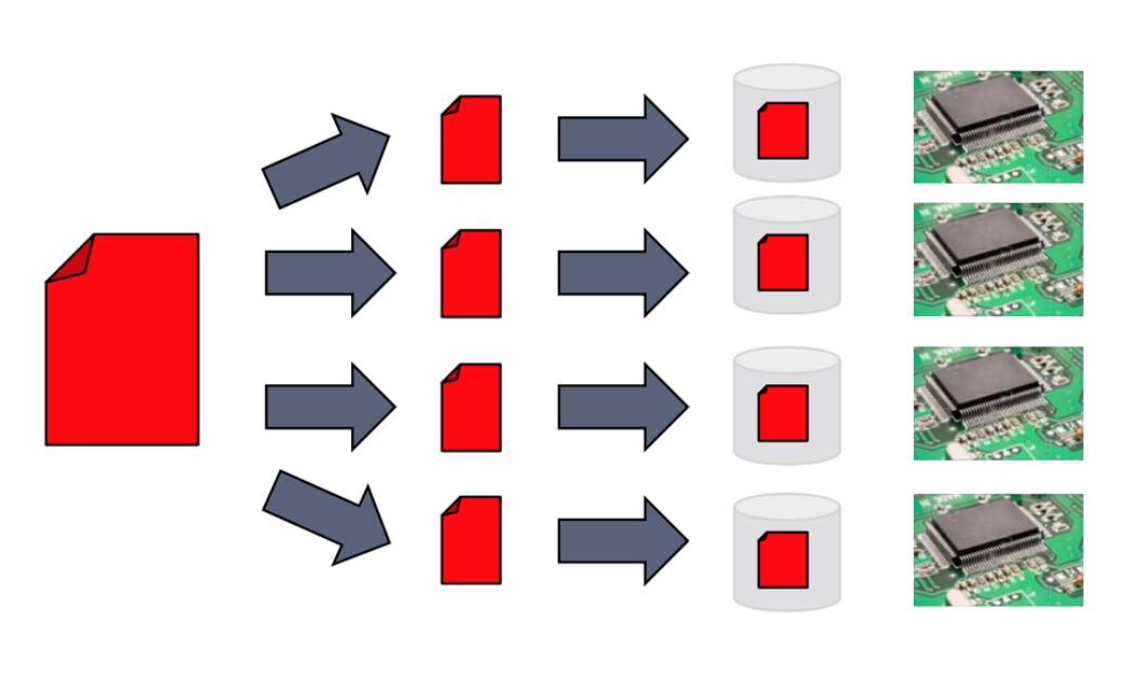
\includegraphics[width=0.8\linewidth]{assets/Screenshot 2026-01-14 at 16.59.53.png}
    \caption{Bottleneck solution for Big Data.}\label{fig:bigdata-bottleneck}
\end{figure}


%
\section{Database per time-series}
I database relazionali classici spesso non bastano, quindi dobbiamo utilizzare dei DB ottimizzati. Se, ad esempio, dobbiamo gestire dati con associati dei ``timestamps'' (ovvero dati con un ordine temporale) si possono usare:
\begin{itemize}
    \item \textbf{InfluxDB}: Specifico per Time Series. I dati sono ordinati fisicamente per tempo. Supporta Retention Policies (cancellazione automatica dati vecchi o aggregazione) e Continuous Queries (query continue su flussi di dati);
    \item \textbf{Cassandra}: Ottimizzato per l'ordinamento basato su timestamp e recupero per intervalli temporali;
    \item \textbf{MongoDB}: Database in origine document-oriented, ma adattabile per serie temporali.
\end{itemize}
Vedi figura \ref{fig:bigdata-timeseries} per la comparazione dei DBMS.

% \begin{figure}
%     \centering
%     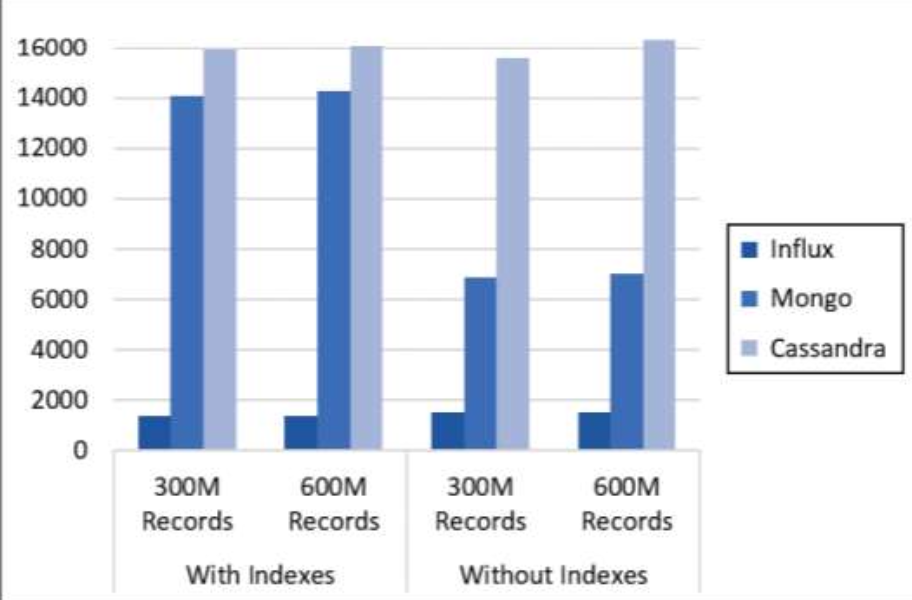
\includegraphics[width=0.6\linewidth]{assets/Screenshot 2026-01-14 at 17.09.07.png}
%     \caption{Tempo (s) per importare 300M e 600M records per ogni DBMS, con e senza indici}\label{fig:bigdata-timeseries}
% \end{figure}

\begin{figure}
    \centering
    \begin{minipage}{0.45\textwidth}
        \centering
        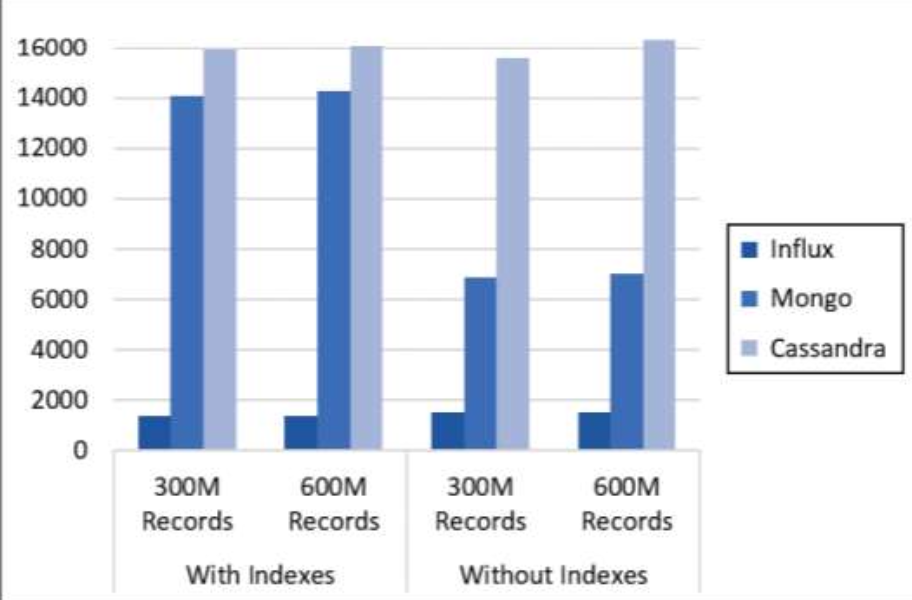
\includegraphics[width=\linewidth]{assets/Screenshot 2026-01-14 at 17.09.07.png}
        \caption{Tempo (s) per importare 300M e 600M records per ogni DBMS, con e senza indici}
        \label{fig:bigdata-timeseries}
    \end{minipage}
    \begin{minipage}{0.45\textwidth}
        \centering
        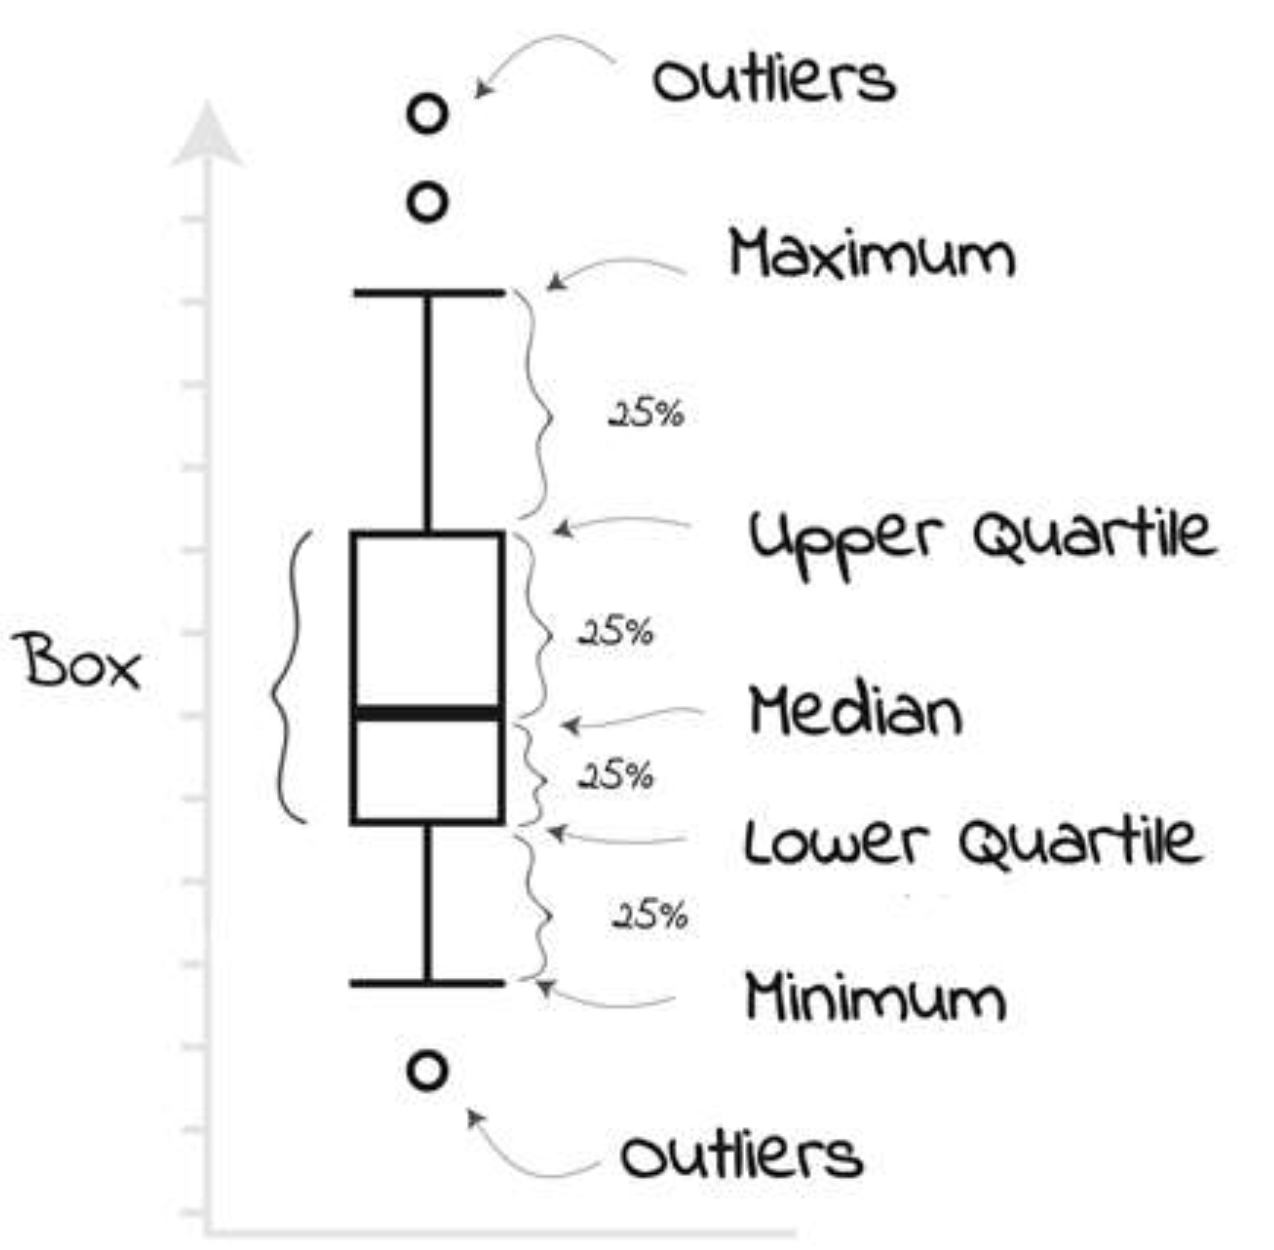
\includegraphics[width=\linewidth]{assets/Screenshot 2026-01-14 at 17.16.37.png}
        \caption{Grafico Box plot}
        \label{fig:bigdata-boxplot}
    \end{minipage}
\end{figure}
%
\section{Data pre-processing}
Prima di poter analizzare i dati bisogna trattarli.
%
\paragraph{Gestione dei missing values} Si possono eliminare gli oggetti difettosi, ignorarli, oppure stimarli (imputazione) basandosi sulla distribuzione di probabilità.
%
\paragraph{Box plot} Strumento grafico fondamentale per visualizzare la distribuzione statistica e identificare gli outliers (valori anomali). Mostra minimo, massimo, mediana, primo quartile (25\%) e terzo quartile (75\%). Vedi figura \ref{fig:bigdata-boxplot} a riguardo.
% \begin{figure}
%     \centering
%     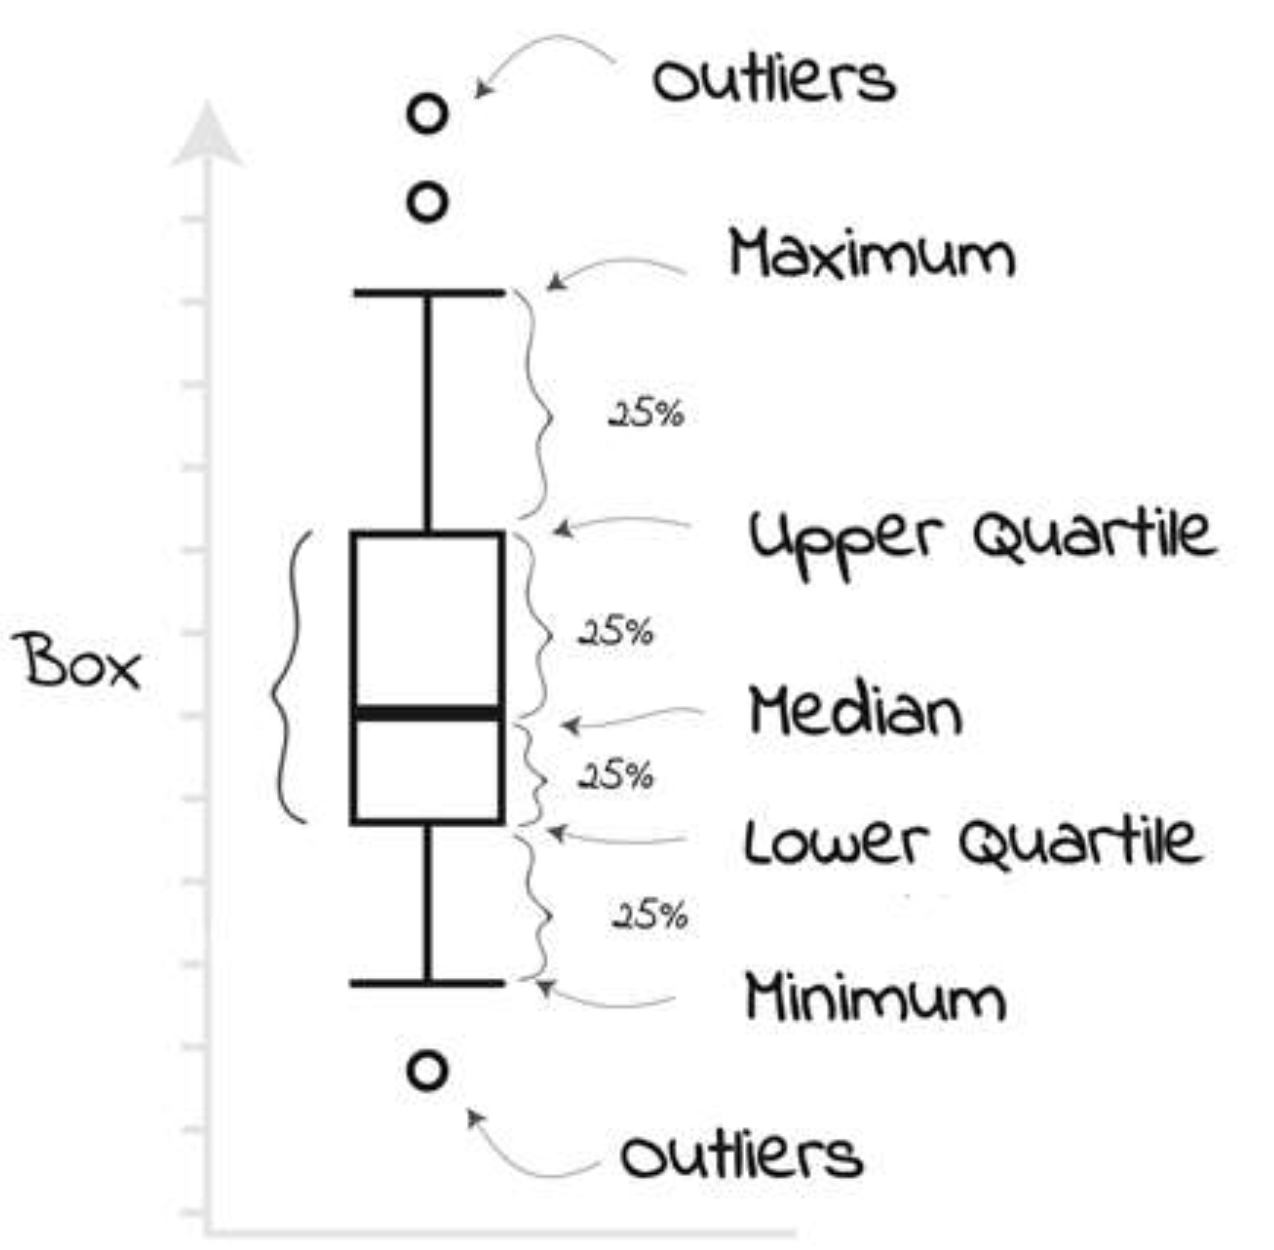
\includegraphics[width=0.5\linewidth]{assets/Screenshot 2026-01-14 at 17.16.37.png}
%     \caption{Grafico Box plot}\label{fig:bigdata-boxplot}
% \end{figure}
%
\paragraph{Correlazione} Misura la forza della relazione lineare tra due variabili (da -1 a +1). Serve a capire quali variabili si influenzano a vicenda (utile per la regressione).
Vedi figura \ref{fig:bigdata-correlation} a riguardo.
\begin{figure}
    \centering
    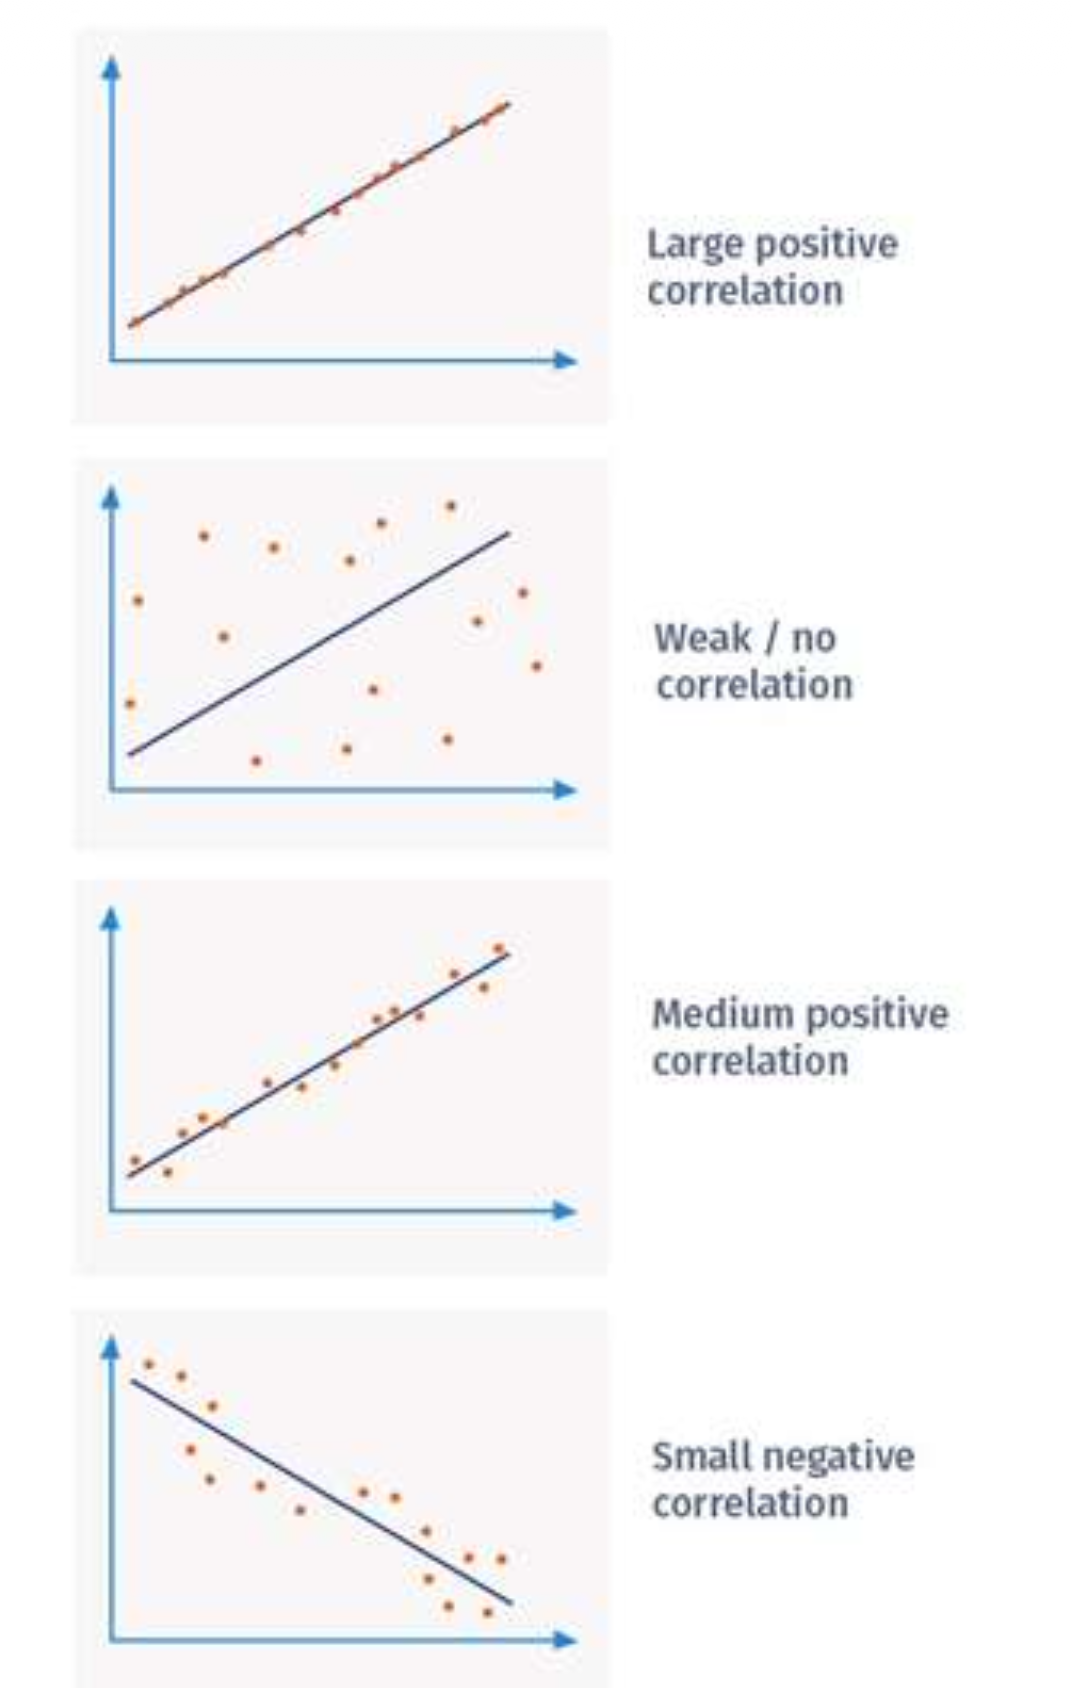
\includegraphics[width=0.4\linewidth]{assets/Screenshot 2026-01-14 at 17.18.22.png}
    \caption{Data Correlation, utilizzato per misurale l'influenza che i dati hanno a vicenda.}\label{fig:bigdata-correlation}
\end{figure}

%
\section{Elaborazione dei dati: data mining}
L'obiettivo è di estrarre informazioni sensate e capibili dai dati, si utilizzano modelli matematici/statistici che identificano patterns nei dati.

Tipi principali di pattern:
\begin{enumerate}
    \item Associazione: Raggruppamenti che si verificano insieme;
    \item Regressione: Prevedere eventi futuri basandosi su quello che è successo nel passato;
    \item Clustering: Scoprire gruppi di dati con comportamenti simili;
    \item Time order: Analisi sequenziale temporale.
\end{enumerate}

%
\section{Visualizzazione dei dati}
Ora che abbiamo i dati elaborati e processati, ci servono strumenti per rendere quest'ultimi comprensibili e supportare decisioni data-driven.
%
\paragraph{Visualizzazione tradizionale (plots)}
Esistono oltre 80 tipi di grafici per la visualizzazione di dati (Bar, Line, Pie, Scatter, Heat Map, ecc.) che possono essere visualizzati sul \href{https://www.datylon.com/blog/types-of-charts-graphs-examples-data-visualization}{Datylon types of charts}.
\begin{example}
    Un esempio può essere il line plot. In questo troviamo come dati la velocità di joint diversi. I buchi nel grafico rappresentano dati mancanti e questo tipo di grafico non ci rende possibile capire la distribuzione e le informazioni statistiche. Vedi figura \ref{fig:visualization-lineplot} a riguardo.
    \begin{figure}
        \centering
        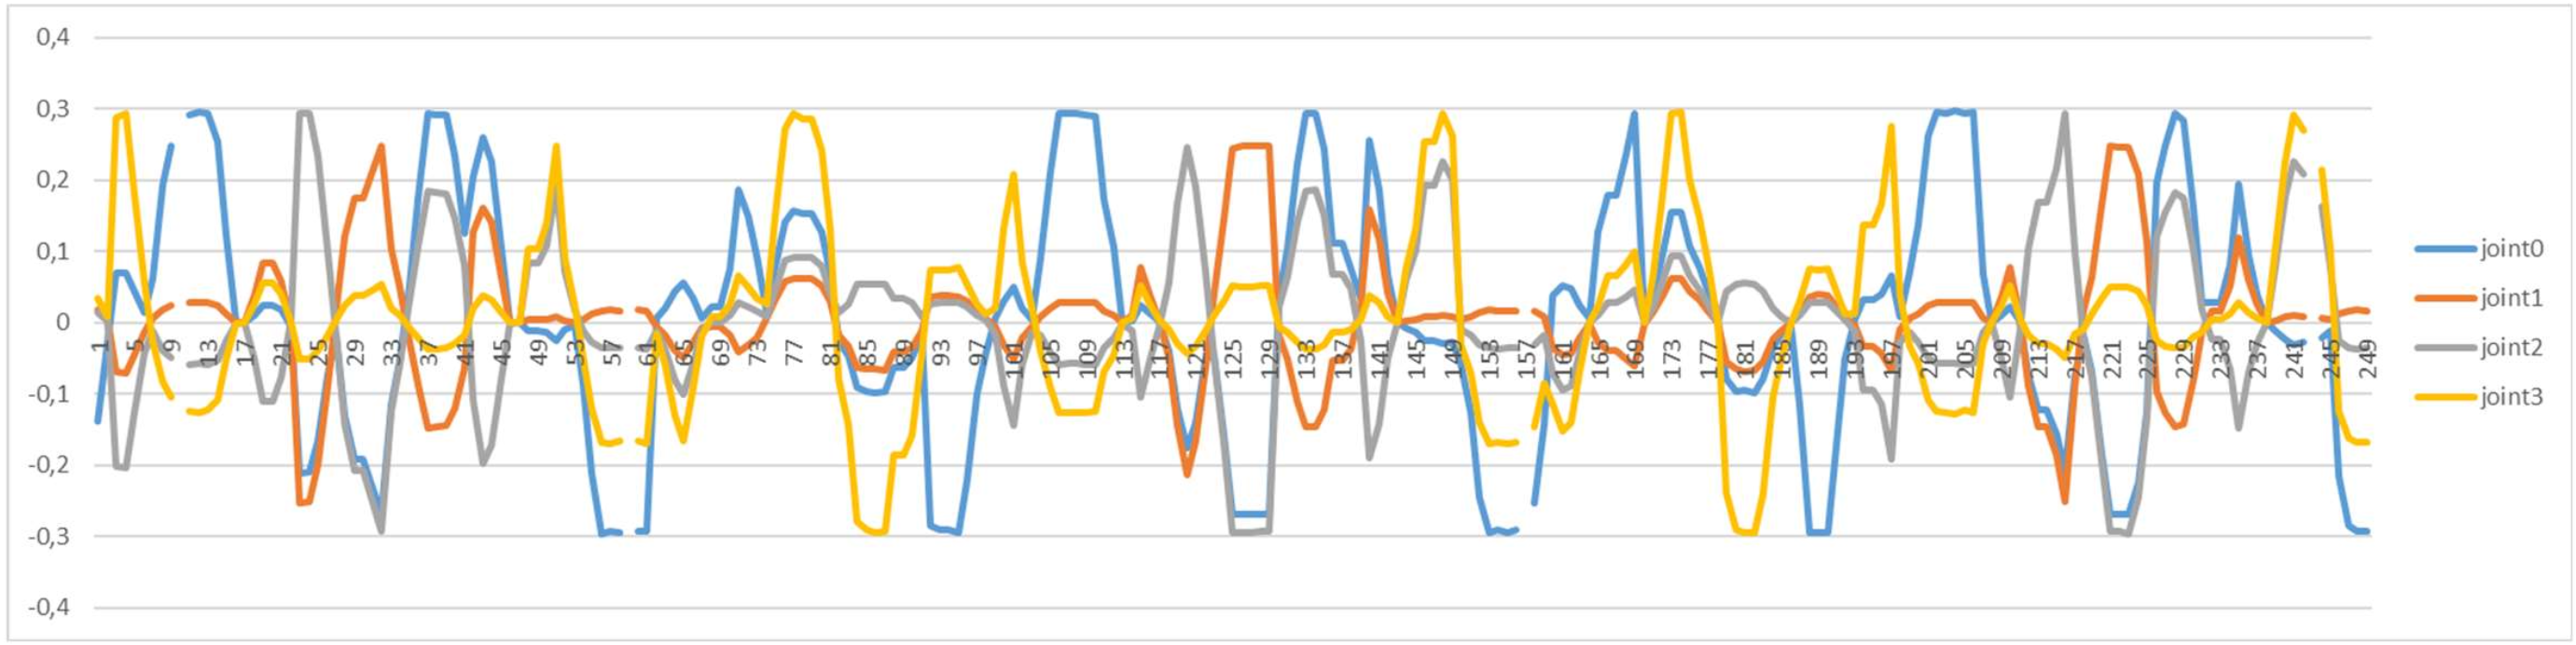
\includegraphics[width=\linewidth]{assets/Screenshot 2026-01-14 at 18.26.36.png}
        \caption{Line plot per la visualizzazione della velocità di 4 joints di un braccio robotico.}\label{fig:visualization-lineplot}
    \end{figure}
\end{example}
%
\paragraph{Visual Analytics} Strumenti interattivi che combinano visualizzazione e analisi profonda, spesso guidati da AI e Machine Learning.
%
\paragraph{Dashboard} Visualizzazione di informazioni importanti in un'unica schermata per una comprensione immediata (es. KPI aziendali, stato dei sensori). Vedi figura \ref{fig:visualization-dashboard} a riguardo.
\begin{figure}
    \centering
    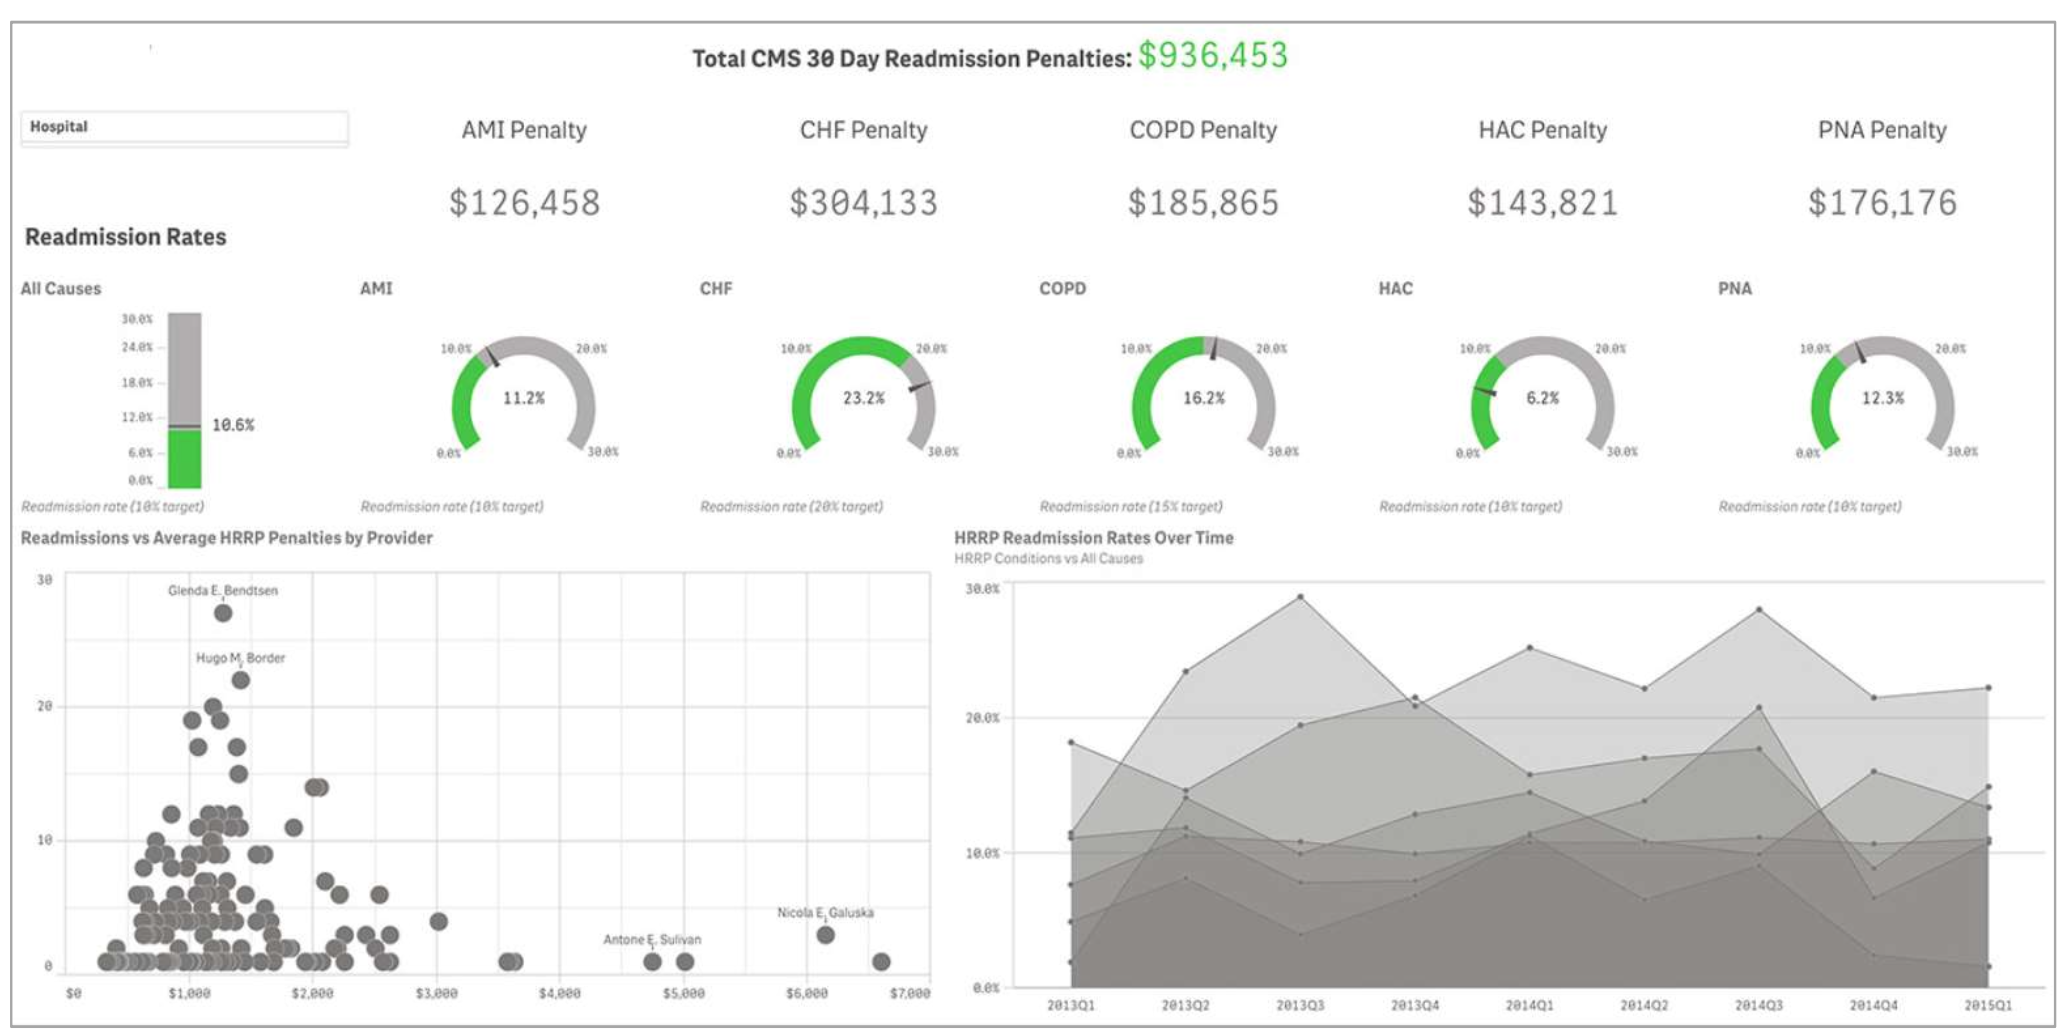
\includegraphics[width=\linewidth]{assets/Screenshot 2026-01-14 at 18.39.47.png}
    \caption{Dashboard per la visualizzazione di dati.}\label{fig:visualization-dashboard}
\end{figure}

%
\section{Sicurezza dei dati}
Mentre i sistemi diventano sempre più interconnessi, ed il livello delle infrastrutture digitali diventa sempre più complesso, i servizi iniziano ad essere vulnerabili a cyber-attacchi:
\begin{quote}{Non ho idea di chi lo abbia detto}
    The system is only as strong as their weakest link.
\end{quote}
%
\paragraph{Vulnerabilità} I dispositivi IoT sono spesso hackerabili se non valutati correttamente.
\begin{itemize}
    \item Possono essere attaccati da hacker e malintenzionati;
    \item Possono ricevere danni per colpa del cambiamento climatico, disastri naturali, vandalismo \dots
\end{itemize}
Alcuni degli attacchi più comuni sono:
\begin{itemize}
    \item Furto di identità/dati: Accesso a informazioni personali;
    \item Hijacking (Dirottamento): Prendere il controllo di un dispositivo (ad esempio dei semafori) per interrompere un processo;
    \item Man-In-The-Middle (MITM): L'hacker intercetta la comunicazione tra due dispositivi fingendosi il mittente (ad esempio inviare falsi dati di ritardo trasporti, rendendo una città in stallo);
    \item DDoS (Distributed Denial of Service): Bombardare la rete di un sistema con pacchetti richieste per rallentarlo o bloccarlo;
    \item Ransomware: Bloccare dati o processi richiedendo un riscatto.
\end{itemize}